\chapter{Space Reduction Approach}
\label{ch:approach}

This part of the thesis discusses the approach to substantially mitigates the space inefficiency characteristic of Hypertrie.  
The technique relies mainly on compressing a Hypertire path with specific characteristics. 
Worth mentioning that the approach does not neglect the other attempts already realized to minimize Hypertrie memory footprint. 
In contrast, it can be considered an added feature that further contributes to the space reduction of the overall Hypertrie data structure. 

\todo{Talk about where my programming work resides?}

\todo{Chapter structure "revisit"}In this chapter, I deliver a motivation to the approach. Afterward, I discuss the new Hypertrie internal nodes' design needed to realize the path compression feature. Finally, algorithms defining the behaviors of the newly designed Hypertrie are also presented. 


\section{Motivation}

Despite its operational efficiency, Hypertrie performance comes not without a trade-off. 
Since Hypertrie is a special kind of a Trie data structure, it inherits some of the fundamental problems of  Tries. 
One of these problems is the excessive space utilization in a worst-case scenario.  \\


The current design and implementation of Hypertrie, however, mitigates the space inefficiency characteristic in two ways. 
First, for each tensor dimension mapping in each node, the Hypertrie uses custom hash map data structures instead of arrays or linked lists to store the keys. 
By using a map, Hypertrie's nodes only stores keys that form prefixes to already existed paths. 
In contrast, arrays utilization in normal Tries considers the whole alphabet set in each node with many array entries store pointers that refer to null\todo{cite!}.  \\

The adoption of maps in Hypertrie also delivers extra performance as looking up keys in a carefully designed map is nearly constant compared to linked list search where it has a linear complexity $O(n)$. 
The other solution realized by Hypertrie to reduce the overall space requirement is to store equal nodes (Subhypertrie) only once. In this way, Hypertrie achieves a moderate level of compression in practice. \\

Despite the previously mentioned attempts to minimize the size of Hypertrie, the excessive memory requirement is still a bottleneck. The case can be witnessed when the set of RDF triples needed to be indexed by Hypertrie increases in size with less overlapping between its elements. As a result, many intermediate nodes store map with a single entry for a particular dimension where the entry hosts a space for key and a pointer. This becomes a space redundancy issue when the leaf node referenced by the pointer has one key only. \\ 

The purpose of the following approach is to try to reach a more space-efficient Hypertrie\todo{Continue here}.

\section{Basic Concept}

The purpose of this section is to give a better intuition on the idea of path compression.  \\

Assuming we want to store the set of RDF triples in listing \ref{lst:example}, presented in Turtle syntax, in our space-efficient Hypertrie: 

\begin{lstlisting}[caption={An example set of RDF triples},label={lst:example}]
@prefix rel: <http://www.example.com/schemas/relationship/> .
@prefix ex: <http://www.example.com/schemas/entities/> .
@prefix xsd: <http://www.w3.org/2001/XMLSchema#> .

ex:Germany rel:capital ex:Berlin .
ex:USA rel:capital ex:Washington_DC
ex:USA rel:political_city ex:Washington_DC
ex:Germany rel:population "82.79e6"^^xsd:integer	
\end{lstlisting}

Tentris do not store the actual values of RDF terms (RTs). Instead, it stores their associated identifiers. 
For generating identifiers, a bijective function $id: RT \to N$ is used. 
For the example of RDF data above, a possible mapping for the terms used is given below: \\

\begin{center}
	\begin{tabular}{ |c|c| } 
		\hline
		$RT$ & $id$ \\
		\hline
		ex:Germany & 17 \\ 
		rel:capital & 4 \\ 
		ex:Berlin & 30 \\ 
		ex:USA & 20 \\
		ex:Washington\_DC & 40 \\
		rel:political\_city & 5 \\
		rel:population & 6 \\
		82.79e6 (integer) & 35 \\
		\hline
	\end{tabular}
\end{center}

\begin{figure}[htbp]
	\centering
	\vspace{-1in}
	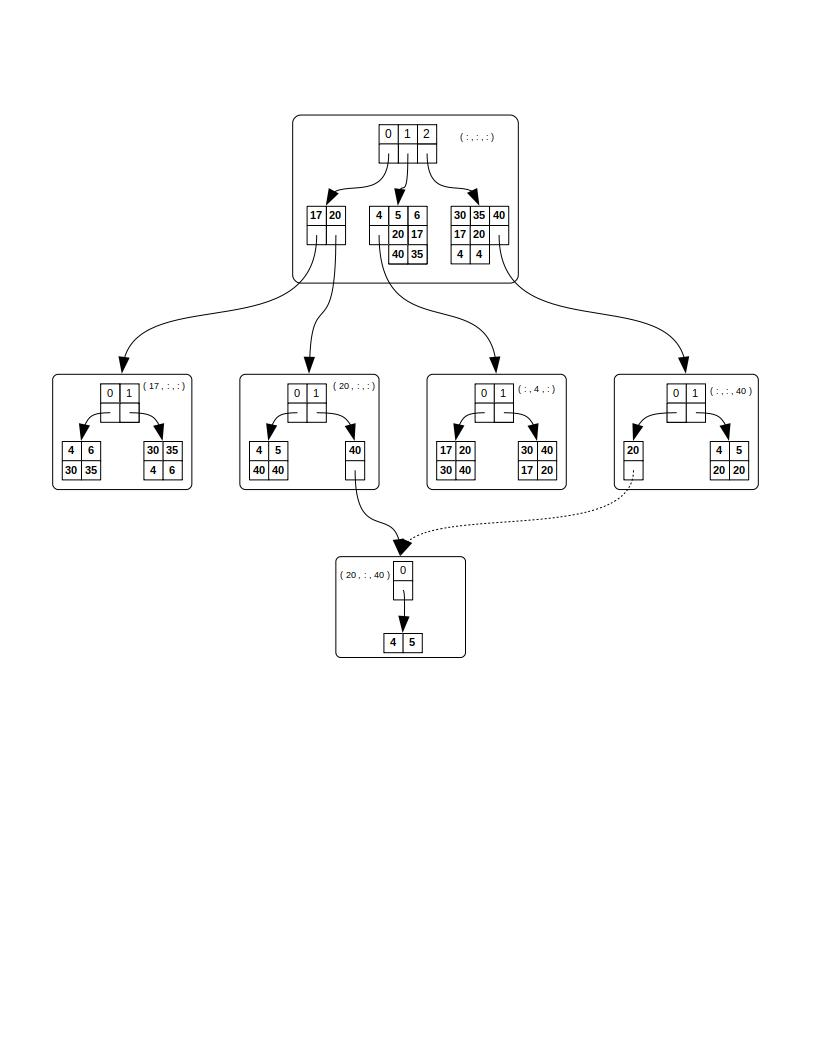
\includegraphics[width=1\textwidth]{figures/example.jpg}
	\caption{Storing RDF in space-efficient Hypertrie}
	\label{fig:example_compressed_trie}
\end{figure}

The Hypertrie will store the triple as shown in Figure \ref{fig:example_compressed_trie},  when the path compression technique is applied. It is straightforward to notice that many keys stored in the second level nodes (depth=2) do not need to be branched further to point to other nodes in the third level. 
As a result, the tree height is cut down, and a substantial amount of memory is saved by storing objects in-place instead of storing them on the heap. 

\todo{talk about the idea of preserving the space saving technique like the one of pointing to an already existed node only once}So, the memory for the pointer to the object on the heap is saved. 
The same method is applied for the root node where keys for a specific dimension are branched by a \textit{lonely path}, i.e. a key path where each element has a single child element. \\

\section{Compressed Hypertrie Nodes}

In order to achieve path compression in Hypertrie, fundamental design changes need to take place. 
By that, we can enable the node to store the entire key suffix\todo{define key suffix}. 
Concretely, each group of Hypertrie nodes in certain tree depth will have their own internal node representation.  \\

We create \textbf{Adaptive Hypertrie nodes}. \\

Concretely, each node must hold internal \textbf{containers} where key suffixes can be stored. \\

We reduce the space requirement of Hypertrie by collapsing Hyptertrie nodes to \textbf{static containers}s. \\

\todo{Talk about the Hypertrie node compressed path container}

From programming point of view, the redesign of Hypertrie nodes' structures is low level. Thanks to C++17 template meta-programming feature, we could separate the compressed nodes realization from the Hypertrie data structure interface. By that, we can still insure a smooth integrity of Hypertrie with other components in Tentris system. \\

\subsection{Features} \todo{Move -> Evaluation chapter with "discussion"}
During the evaluation phase, I will prove that the performance of the space efficient Hypertrie is at least as much as the performance of the base (reference) Hypertrie. 
The compressed Hypertrie is \textbf{cache-conscious}. 
That is the frequently accessed compressed key paths suffixes stored at the root node in array-based containers will increase the probability that those paths resides within cache. 

\subsection{Internal Node Representations}

Now I come to the part where the internal structure of space-efficient Hypertrie nodes are discussed. 
In my approach, it is a requirement to realize the container concept for each node\footnote{Leaf nodes are not considered.} . 
As a result, each inner node should still be able to expand at certain edges to sub Hypertrie nodes while maintaining a compressed key path in its bounded container for other edges. \\

The compressed key path container implementation varies depending on the node depth. 
The idea of having different internal representations comes from the fact that, based on the current structure of nodes on depth two, I found that there is no need to add an additional structure that serves as a container for the key path. \todo{smaller sentences with less pronoun}
Instead, I exploit the space dedicated to pointer value existed as a value in the hash table\todo{discuss the existence of Hypertire structure} of store the compressed key path.\todo{ALEX: is this sentence scientifically accurate?} \\ 

\todo{ALEX: Why using tagged pointer for internal nodes saves space (hash tables already have initial space values? Answer: Yes)}

Since Hypertrie's internal nodes can be either a root node or depth two nodes, we can distinguish two variants of internal node representations: 

\subsubsection{Depth 3 Node (root node)} 
%As the Hypertrie has a predefined fixed depth $d = 3 $, There exists a single root node. 
In addition to the set of edges (hash tables) $HT_{3,p}$ for each position $p \in P = \{0, 1, 2\}$, the root node also holds another array of hash tables $CommHT_{p}$ that maps key parts $k_{j}$ to static arrays $arr_{j}$. 
Each array will serve as the container for the key path prefixed by the associated key part $k_{j}$ at the corresponding position $p$ as depicted in Fig. \ref{fig:compressed_depth_3_node}. 
We call the edges $k_{j}$ stored  in $CommHT_{p}$ \textbf{compressed edges}. Clearly, a key part at a particular position $p$ can either represents a compressed or non-compressed edge at a time, so it exists in either $HT_{p}$ or $CommHT_{p}$. 
The remaining key path $k_{S} = <k_{1}, k_{2}>$ associated with each compressed edge $k_{j}$ holds the key part chain ordered by their presence in the key. \\

Worth to mention that the key path associated with each compressed edge still represents a $2D$ sparse tensor $S$ that results from slicing tensor $T$ represented by the root node at position $p$ with key part $k_{j}$. The resultant tensor $S$ has a single entry $<k_{1}, k_{2}>$ that evaluates to $1$. 
As a result, it is important to maintain the order of the elements in the compressed path $arr_{j}$ as each key $arr[i]$ represents the single edge at position $i$ in $S$ whose child is the other array entry. \\

\subsubsection{Depth 2 Node} Internal nodes with $d=2$ realize the static container concept associated with compressed edges differently than for the root node. 
\todo{Talk about hash table capacity}
Considering the number of internal nodes, it becomes unfeasible, assigning an extra set of hash tables for each node that serve as key part chains containers. \\

To realize the container concept, we exploit the fact that key suffixes for edges in $d=2$ node comprise a single key part.
Hence, we could reuse the space already booked to store the pointers to child nodes (leafs) to hold the suffixed key part.
For the pointer $ptr_{j}$ associated with the edge $k_{j}$ to serve the purpose of either pointing to a child node or holding an integer value, we make it a tagged pointer (cf. \ref{sec:preliminaries:pointertagging}). \\

Consequently, child pointers $ptr_{j} = (value, tag)$ for edges in depth=2 nodes carry two pieces of information. (1) A $value$  where either an address or integer value is held. (2) A $tag$ that indicates whether the associated edge $k_{j}$ is compressed or non-compressed. Figure \ref{fig:compressed_depth_2_node} visualizes the structure.

\subsubsection{Node Expansion}

\subsubsection{Virtual Nodes}

\begin{figure}
	\centering
	\vspace{-0.3in}
	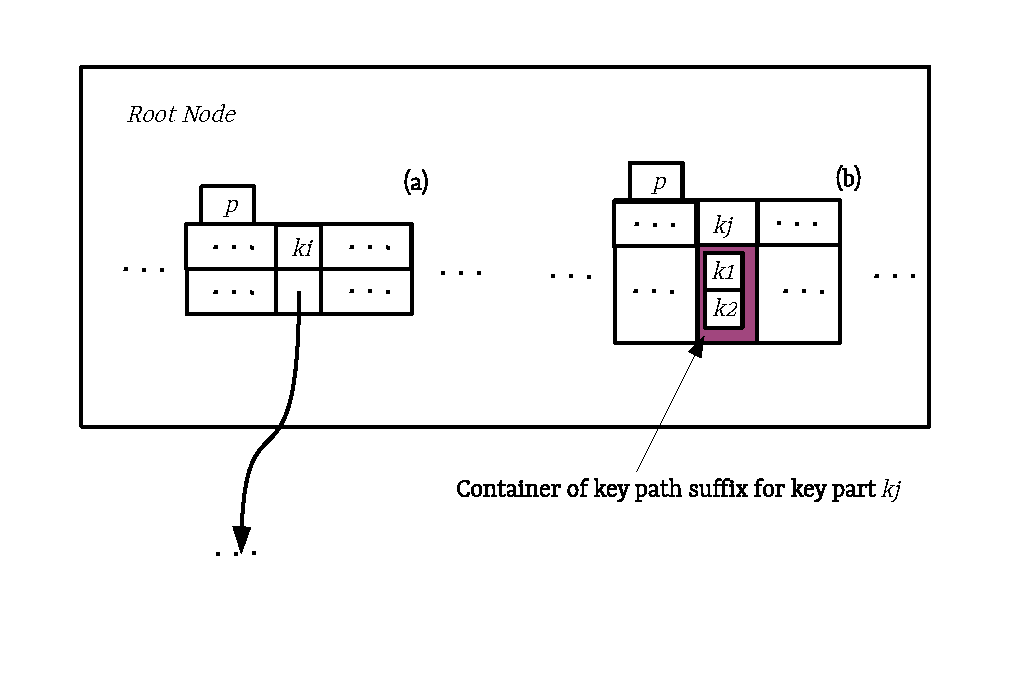
\includegraphics{figures/chapter4/depth3}
	\caption{Depth 3 Node}
	\label{fig:compressed_depth_3_node}
\end{figure}



\begin{figure}
	\centering
	\vspace{-1in}
	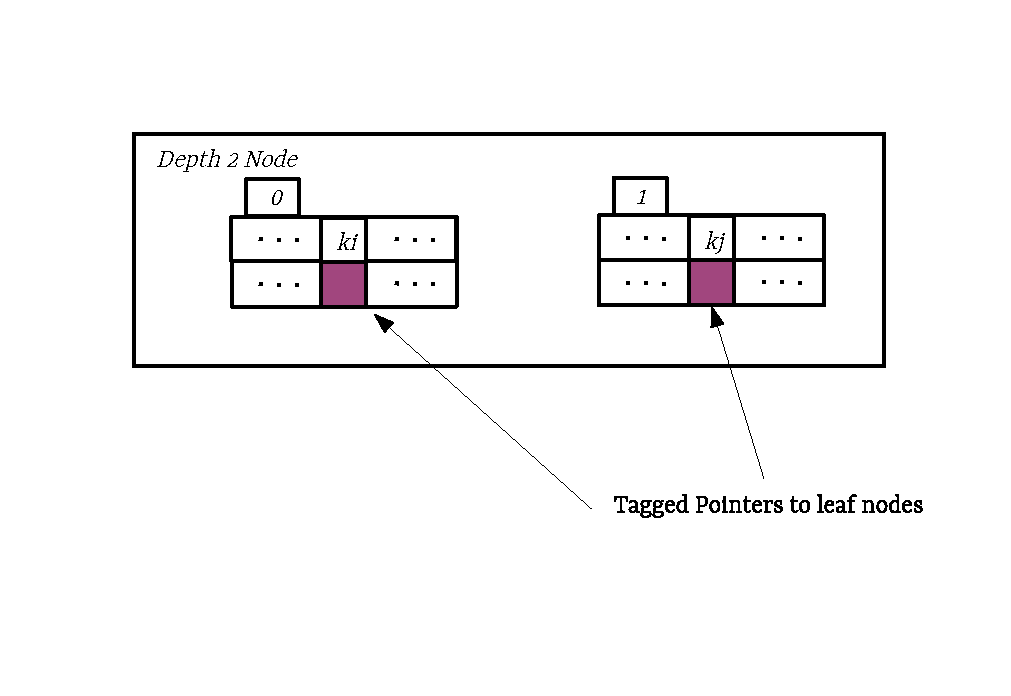
\includegraphics{figures/chapter4/depth2}
	\caption{Depth 2 Node}
	\label{fig:compressed_depth_2_node}
\end{figure}

\section{Algorithms}
This is a text for algorithms

\paragraph{Key Insertion} 
\paragraph{Key Retrieval}
\paragraph{Slicing} 

\paragraph{Diagonal}

\section{Storage Discussion}

\todo{ALEX: Whether we skip that to the evaluation}
Best case is easy. all triples are stored in the root node???

